\documentclass[]{article}
\usepackage{proceed2e}
\usepackage{enumerate}
\usepackage{algpseudocode}
\usepackage[ruled]{algorithm}
\usepackage{url}
\usepackage{framed}
\usepackage{amsfonts,amsmath,amsthm,amssymb}
\usepackage{graphicx}
\usepackage{url}
\usepackage{color}

\newcommand {\mean} {\ensuremath {\mathop{\mathrm{mean}}}}
\newcommand {\median} {\ensuremath {\mathop{\mathrm{median}}}}
\newcommand {\N} {\ensuremath {\mathcal{N}}}
\newcommand {\IE} {\ensuremath {\mathbb{E}}}
\newcommand {\cov} {\ensuremath {\mathop{\mathrm{cov}}}}
\newcommand {\BEL} {\ensuremath {\mathop{\mathrm{BEL}}}}

\newtheorem{dfn}{Definition}
\newtheorem{thm}{Theorem}
\newtheorem{lmm}{Lemma}
\newtheorem{crl}{Corollary}

\begin{document}


\section{Upper Bounds on Value of Information}

The intrinsic VOI $\Lambda_i$ of pulling an arm is the expected decrease
in the regret compared to selecting the best arm without pulling any arm at
all. Two cases are possible:
\begin{itemize}
\item the arm $\alpha$ with the highest sample mean $\overline
  X_\alpha$ is pulled, and $\overline X_\alpha$ becomes lower than
  $\overline X_\beta$ of the second-best arm $\beta$;
\item another arm $i$ is pulled, and $\overline X_i$ becomes higher
than $\overline X_\alpha$.
\end{itemize}
The \textit{myopic} VOI estimate is of limited applicability to
Monte-Carlo sampling, since the effect of a single sample is small,
and the myopic VOI estimate will often be zero. However, for the
common case of a fixed budget of samples per node, $\Lambda_i$ can be
estimated as the intrinsic VOI $\Lambda_i^b$ of pulling the $i$th arm
for the rest of the budget.  Let us denote the current number of
samples of the $i$th arm by $n_i$, and the remaining number of samples
by $N$:
\begin{thm} $\Lambda_i^b$ is bounded from above as
\begin{align}
\label{eqn:thm-be}
  \Lambda_\alpha^b& \le \frac {N \overline X_\beta^n} {N+n_\alpha}\Pr(\overline X_\alpha^{n+N}\le\overline X_\beta^n)\nonumber\\
    &\le \frac {N \overline X_\beta^n} {n_\alpha} \Pr(\overline X_\alpha^{n+N}\le\overline X_\beta^n)\nonumber\\
\Lambda_{i|i\ne\alpha}^b& \le \frac{ N(1-\overline  X_\alpha^{n_i})} {N+n_i}\Pr(\overline X_i^{{n_i}+N}\ge\overline X_\alpha^{n_i})\nonumber\\
     &\le \frac {N(1-\overline X_\alpha^{n_i})} {n_i}\Pr(\overline   X_i^{{n_i}+N}\ge\overline X_\alpha^{n_i})
\end{align}
\label{thm:be}
\end{thm}

The probabilities can be bounded from above using the
Hoeffding inequality \cite{Hoeffding.ineq}:
\begin{thm} The probabilities in equations (\ref{eqn:thm-be}) are bounded from above as
\begin{align}
  \label{eqn:probound-blnk-hoeffding}
  \Pr&(\overline X_\alpha^{{n_\alpha}+N} \le \overline X_\beta^{n_\alpha})
  \le 2\exp\left(- \varphi(n_\alpha)(\overline X_\alpha^{n_\alpha} - \overline X_\beta^{n_\alpha})^2 n_\alpha
  \right)\nonumber\\
  \Pr&(\overline X_{i|i\ne\alpha}^{n+N} \ge \overline X_\beta^n)
  \le 2\exp\left(- \varphi(n_i) (\overline X_\alpha^n -\overline  X_i^n)^2 n_i \right)
\end{align}
where $\varphi(n)=2(\frac {1+n/N} {1+\sqrt {n/N}})^2 > 1.37$.
\label{thm:hoeffding-prob-bounds}
\end{thm}
\begin{crl}
An upper bound on the VOI estimate $\Lambda_i^b$ is obtained
by substituting (\ref{eqn:probound-blnk-hoeffding}) into (\ref{eqn:thm-be}).
\begin{align}
  \label{eqn:bound-blnk-hoeffding}
  \Lambda&_\alpha^b \le \hat\Lambda_\alpha^b=\frac {2N\overline X_\beta^{n_\alpha}} {n_\alpha}\exp\left(- 1.37(\overline X_\alpha^{n_\alpha} - \overline X_\beta^{n_\alpha})^2 n_\alpha\right)\nonumber\\
  \Lambda&_{i|i\ne\alpha}^b\le \hat\Lambda_i^b=  \frac {2N(1-\overline  X_\alpha^{n_i})} {n_i}\exp\left(- 1.37(\overline X_\alpha^{n_i} - \overline X_i^{n_i})^2 n_i\right)
\end{align}
\label{crl:bound-blnk-hoeffding}
\end{crl}
Better bounds can be obtained through tighter estimates on the
probabilities, for example, based on the empirical Bernstein
inequality~\cite{MaurerPontil.benrstein}, or through a more careful
application of the Hoeffding inequality.

\section{VOI-based Sampling Control}

\subsection{Selection Criterion}

Following the principles of rational metareasoning, an arm with the
highest VOI should be pulled at each step. The upper bounds
established in Theorem~\ref{thm:be} can be used as VOI estimates. MCTS
differs from pure exploration in Multi-armed Bandits in that the
distributions of the rewards are not stationary. However, VOI
estimates computed as for stationary distributions work well in
practice. As illustrated by the empirical evaluation. As illustrated
by the empirical evaluation (Section~\ref{sec:empirical-evaluation}),
estimates based on upper bounds on the VOI result in rational sampling
policies, and exhibit performance comparable to the performance of
some state-of-the-art heuristic algorithms.

\subsection{Termination Condition}
\label{sec:control-termination-condition}

The simplest termination condition for a sampling policy is the
budget---a fixed number of samples performed before a decision is
made. When a sample has a cost commensurable with the value of
information of a measurement, an upper bound on the intrinsic VOI can
be used to stop the sampling if the intrinsic VOI of any action
is less than the cost of sampling $C$:
\begin{equation}
\mbox{stop if } \max_i \Lambda_i \le C
\end{equation}
Blinkered VOI estimates~(\ref{eqn:thm-be},
\ref{eqn:bound-blnk-hoeffding}) include the remaining budget $N$ as a
factor, but given the cost of a single sample $c$, the cost of the
remaining samples accounted for in estimating the intrinsic VOI is
$C=cN$. $N$ can be dropped on both sides of the inequality,
and a viable stopping condition is
\begin{align}
\frac 1 N \Lambda_\alpha^b \le&\frac {\overline X_\beta^{n_\alpha}}
  {n_\alpha}\Pr(\overline X_\alpha^{n_\alpha+N}\le\overline
  X_\beta^{n_\alpha})\le c\nonumber\\
\frac 1 N \max_i\Lambda_i^b\le &\max_i\frac {(1-\overline X_\alpha^{n_i})} {n_i}\Pr(\overline
  X_i^{n_i+N}\ge\overline X_\alpha^{n_i})\le c\nonumber\\
    &\forall i: i\ne\alpha
\label{eqn:stopping-blnk}
\end{align}
The empirical evaluation (Section~\ref{sec:empirical-evaluation})
confirms viability of this stopping condition and illustrates the
influence of the sample cost $c$ on the performance of
the sampling policy.

\subsection{Sample Redistribution in Trees}
\label{sec:control-redistribution}

Monte-Carlo tree search \cite{Chaslot.montecarlo} selects at each
search step an action that appears to be the best based on outcomes
of \textit{search rollouts}. Two different criteria are employed in
action selection during a rollout:
\begin{itemize}
\item at the first step, the value of partial
information should be maximized to minimize the \textit{simple} regret
of the selection at the current root node;
\item as the goal of sampling in deeper tree nodes is estimating the
value of a node, rather than selection, it makes sense to minimize
the \textit{cumulative} regret of the rollouts from the second step
onwards.
\end{itemize}

A natural approach would be to apply an algorithm that minimizes the
simple regret in Multi-armed bandits at the first step, and the
cumulative regret during the rest of the rollout.  However, this
approach assumes that the information obtained from rollouts in the
current state is discarded after an action is selected. In practice,
many successful Monte-Carlo tree search algorithms re-use rollouts
originating from an earlier search state and passing through the
current search state; thus, the value of information of a rollout is
determined not just by the influence on the choice of the action at
the current state, but also by the influence on the choice at future
search states, provided the rollout passes through the search states
which will be visited.

One way to account for this re-use would be to incorporate the
`future' value of information into a VOI estimate. However, this 
approach appears to be complicated. Alternatively, one can behave
myopically in search tree depth:
\begin{enumerate}
\item estimate VOI as though the information is discarded after each step;
\item stop early if the VOI is below a certain threshold
   (see Section~\ref{sec:control-termination-condition});
\item save the unused sample budget for search in future state, such that
   if the nominal budget is $N$, and the unused budget in the last state
   is $N_u$, the search budget in the next state will be $N+N_u$.
\end{enumerate}
In this approach, the cost of a sample in the current state is the
VOI of increasing the budget of a future state by one sample.  It is
unclear whether this cost can be accurately estimated, but supposedly
a fixed value for a given problem type and algorithm implementation
would work. Indeed, the empirical evaluation (Section~\ref{sec:emp-go})
confirms that stopping and sample redistribution based on a learned
fixed cost  substantially improve the performance of the VOI-based
sampling policy in game tree search.

\section{Empirical Evaluation}
\label{sec:empirical-evaluation}

\subsection{Selecting The Best Arm}
\label{sec:emp-arm}

\begin{figure}[h!]
\centering
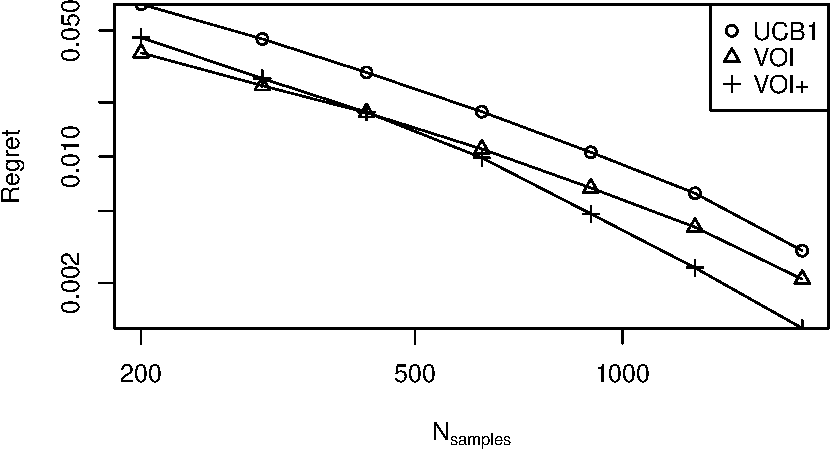
\includegraphics[scale=0.6]{flat.pdf}
\caption{Random instances: regret vs. number of samples}
\label{fig:random-instances}
\end{figure}

The sampling policies are first compared on random Multi-armed bandit 
problem instances. Figure~\ref{fig:random-instances} shows results for
randomly-generated Multi-armed bandits with 32 Bernoulli arms, with
the mean rewards of the arms distributed uniformly in the range~$[0,
  1]$, for a range of sample budgets~$32..1024$, with multiplicative
step of~$2$. The experiment for each number of samples was repeated
10000 times. UCB1 is always considerably worse than the
VOI-aware sampling policy.

\subsection{Playing Go Against UCT}
\label{sec:emp-go}

The policies were also compared on Computer Go, a  search domain
in which UCT-based MCTS has been particularly successful
\cite{Gelly.mogo}. A modified version of Pachi \cite{Braudis.pachi}, a state of the art
Go program, was used for the experiments:
\begin{itemize}
\item The UCT engine of Pachi was extended with VOI-aware sampling
  policies at the first step. 
\item The stopping condition for the VOI-aware policy was
  modified and based solely on the sample cost, specified as
  a constant parameter. The heuristic stopping condition for the
  original UCT policy was left unchanged.
\item The time-allocation mode based on the fixed number of samples
  was modified for \textit{both the original UCT policy and the VOI-aware
  policies} such that 
  \begin{itemize}
    \item the same number of samples is available to
      the agent at each step, independently of the number of pre-simulated
      games;  
    \item if samples were unused at the current step,
      they become available at the next step. 
  \end{itemize}
\end{itemize}
While the UCT engine is not the most powerful engine of Pachi, it is still a strong
player. On the other hand, additional features of more advanced
engines would obstruct the MCTS phenomena which are the subject of
the experiment.
\begin{figure}[h!]
\centering
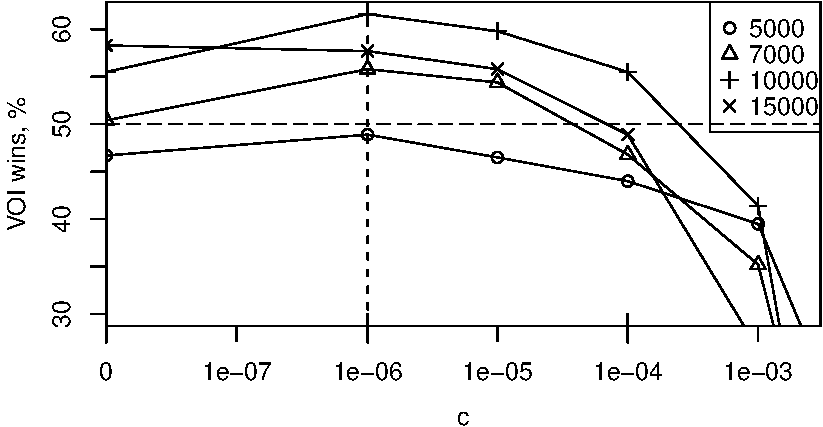
\includegraphics[scale=0.6]{uctvoi.pdf}
\caption{Go: winning rate vs. $c$}
\label{fig:uctvoi}
\end{figure}
The engines were compared on the 9x9 board, for 5000, 7000, 1000, and
15000 samples (game simulations) per ply, each experiment was repeated
1000 times. Figure~\ref{fig:uctvoi}
show the winning rate of UCT against the VOI-aware policy
vs. the stopping threshold $c$ (if the maximum VOI of a sample is below
the threshold, the simulation is stopped, and a move is chosen). Each
curve in the figure corresponds to a certain number of samples per
ply. For the stopping threshold of $10^{-6}$, the VOI-aware policy
is almost always better than UCT, and  reaches the winning rate of
64\% for 10000 samples per ply.

\begin{figure}[h!]
\centering
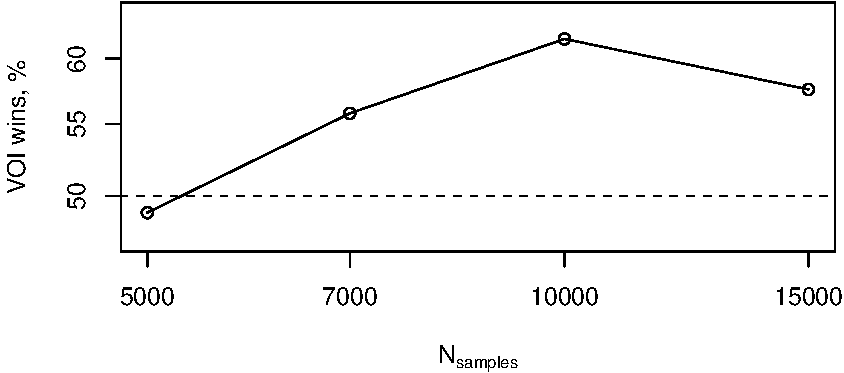
\includegraphics[scale=0.6]{voi-wins.pdf}
\caption{Go: winning rate for $c=10^{-6}$}
\label{fig:voi-wins}
\end{figure}

Figure~\ref{fig:voi-wins}
shows the winning rate of VOI against UCT vs. the number of
samples for $c=10^{-6}$. In agreement with the intuition
(Section~\ref{sec:control-redistribution}), VOI-based stopping and
sample redistribution is most influential for medium numbers of
samples per ply. When the maximum number of samples is too low, early
stopping would result in poorly selected moves. On the other hand,
when the maximum number of samples is sufficiently high, the VOI of
increasing the maximum number of samples in a future state is low.

\bibliographystyle{plain}
\bibliography{refs}


\end{document}
